\chapter{Combustion Model}
\section{Premixed ozone oxygen laminar flame model}
We shall use Heimerl and coffee's contemporary method for modelling combustion flame problem. A one dimensional, premixed, laminar, steady state ozone oxygen flame was considered in their theortical model. The reason for choosing this model was due to its simplicity. The chemical reactions involved only three species 


			$$O_3 + M \rightleftharpoons O + O_2 + M $$
			$$ O + O_3 \rightleftharpoons A_2  2O_2$$ 
			$$A + AB \rightleftharpoons A_2 + B$$
\noindent Where M represents the third body which could be either $O$, $O_2$ or $O_3$. 

\noindent The species conservation equation is given as 
\begin{eqnarray}
	\frac{\partial \rho_i}{\partial t} + \nabla . (\rho_i v) &= \nabla . (\rho D_{ij} \nabla Y_i) + w_i
\end{eqnarray}
\noindent Where, the rate of production for species $i$ is given by the following 
	
Where $$w_i = Mw_i \sum_{k=1}^{6}(v_{k,i}^{''} - v_{k,i}^{'}) B_k T^{\alpha_k} e^{\frac{-E_a}{R_u T}} \prod_{j=1}^3 \left(\frac{X_j p}{R T} \right)^{v'_{j,k}}$$

\noindent The above equation considers all 6 reactions for all the three species. 

\noindent From atomic species conservation 
	$$\sum_{i=1}^{N} v_i{'}M_i \rightleftharpoons \sum_{i=1}^{N} v_i{''}M_i $$
\noindent Where $E_a$ is the activation energy, $R_u$ is the universal gas constant, $X_j$ is the molar concentration of the reactant j, $Mw_i$ is the molecular weight of the reactant. $v'_{j,k}$ is the moles of reactant j in the reaction k. $v''_{j,k}$ is the number of moles of product. 

\bigskip

\noindent The overall continuity equation, species conservation equation and energy conservation equation are solved to calculate the flame paraneters. The energy equation considers that the pressure is constant throughout the reaction zone. The viscous dissipation is negligible and there is no body force work. 

\noindent The Diffusion equation is given 
\begin{eqnarray}
\frac{\partial X_k}{\partial x} &= \sum_{j=1}^{3} \frac{X_k X_j}{D_{jk}} (V_j - V_k)
\end{eqnarray}

\noindent Where $D_{jk}$ is the fick's diffusion coefficient. $V$ is the diffusion velocities. 

\noindent The boundaries are defined by specifying the concentration of $O_3$, $O_2$ at the inlet. 

\section{The experimental data on laminar flame speed}

To compare our results we have used the experimental data given by the A.G.  streng and A.V. Grosse, They have done experiments with ozone flame in tube and ozone flame on the tip of the burner. We will be using the results of the later. They have shown that laminar flame speed or burning velocity varies with the initial concentration of the ozone. The table given below shows the burning velocity with respect to initial concentration of the ozone. We concentrate on two speciifc cases where initial concentration of ozone is 53 percent and 100 percent. The laminar flame speed for 53 percent is measured in the burner with inner diameter 1.3mm  and rate of 7.7 cc/sec. The laminar flame speed for 100 percent ozone is taken on .66 inner diameter tip 0.66 mm and the flow rate of 8.23 cc/sec. 
The measured laminar flame speed is given below. Laminar flame measurements are carried out at 300K and 1 atmosphere pressure. 

\begin{table}[h]
\caption {Experimental laminar flame speed given by A.G. Streng and A.V. Grosse} \label{tab:title}
\begin{center}

\begin{tabular}{|c|c|}
\hline
 \textbf{ Initial Concentration of $O_3$ ($\pm 0.2 \% )$}  &  \textbf{ Laminar Flame Speed (cm/s)} \\ \hline
 17& 9.2 \\  \hline
 20& 18.2 \\ \hline
 28& 52.2 \\ \hline
 40& 125 \\  \hline
 46&  166 \\ \hline
 53&  210 \\ \hline
 75&  331 \\ \hline
100&  475 \\ \hline
\end{tabular}
\end{center}
\end{table}

\section{Geometry with boundary conditions}

\begin{figure}[h!]
  
  \centering
   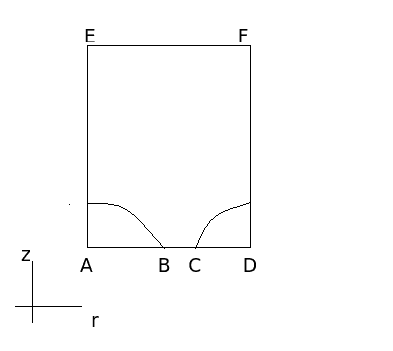
\includegraphics[scale=0.5]{geometricbcs}
   \caption{Geometry}
\end{figure}
\begin{itemize}
\item $AB$ is the inlet
\item $BC$ is the thickness of the burner tube
\item $CD$ is the outside of the burner
\item $DE,EF$ is the domain of interest
\item $AE$ is the Axisymmetric line
\end{itemize}

\bigskip
\noindent The following assumption are made
\begin{itemize}
\item At the inlet, the incoming velcity has parabolic profile. i.e poissuelle flow. 
\item The surface chemistry at the wall of the burner is neglected. 
\item At the outside of the burner, the incoming air has couette flow profile. 
\item $DE,EF$ are the boundaries of the domain. No change occurs after this point. 
\end{itemize}
	
\noindent The boundary conditions are defined as follows 
\bigskip

\noindent At the inlet ($AB$)
\begin{itemize}
\item $u_r = 0$ and $u_z=5801.9 mm/s$
\item $C_i = 1$ 
\item $T = 300K$
\item $p=1 atmos$
\end{itemize}

\bigskip 
\noindent On $BC$
\begin{itemize}
\item $u_r = 0$ and $u_z=0 mm/s$
\item $\frac{\partial C_i}{\partial r} =0 $ and $\frac{\partial C_i}{\partial z} =0 $
\item $T = 300K$
\item $p=1 atmos$
\end{itemize}

\noindent On $CD$
\begin{itemize}
\item $u_r = 0$ and $u_z=5801.9 mm/s$
\item $ C_{O_2} =21 \% $
\item $T = 300K$
\item $p=1 atmos$
\end{itemize}

\noindent On $DF$ and $FE$
\begin{itemize}
\item $\frac{\partial u_r}{\partial r} =0 $ and $\frac{\partial u_z}{\partial z} =0 $
\item $\frac{\partial C_i}{\partial r} =0 $ and $\frac{\partial C_i}{\partial z} =0 $
\item $\frac{\partial T}{\partial r} =0 $ and $\frac{\partial T}{\partial z} =0 $
\item $\frac{\partial p}{\partial r} =0 $ and $\frac{\partial p}{\partial z} =0 $
\end{itemize}


\noindent On $AF$
\begin{itemize}
\item $\frac{\partial u_r}{\partial r} =0 $ 
\item $\frac{\partial C_i}{\partial r} =0 $ 
\item $\frac{\partial T}{\partial r} =0 $  
\item $\frac{\partial p}{\partial r} =0 $
\end{itemize}







